\subsection{What is Drools?}

JBoss Rules, or as it is more commonly known, Drools, is the leading opensource rules engine written in Java.
In this paper when we use the name "Drool" we are referring to the "Drools Expert" which is the rule engine module of the Drools Suite.
Drools started in 2001, but rose to prominence with it's 2005 2.0 release.  
It is an advanced inference engine using an enhanced version of the Rete algorithm, called Rete\-OO\cite{sottara2010configurable}, adapted to an object-oriented interface specifically for Java.
Designed to accept pluggable language implementations, it can also work with Python and .Net.
It is considered one of the most developed and supported rules platforms.

For rules to be executed there are 4 major components as demonstrated in figure \ref{fig:Drools_components}.
The production memory contains the rules.  
This will not change during an analysis session.
The rules are the focus of this thesis and therefore we will delve into much more detail later on these.

In Forgy's\cite{forgy1989rete} overview of a rete algorithm, the following steps occur.
\begin{enumerate}
    \item Match : Evaluate the LHSs of the productions to determine which are satisfied given the current contents of working memory
    \item Conflict resolution : Select one production with a satisfied LHS; if no productions have satisfied LHSs, halt the interpreter
    \item Act : Perform the actions in the RHS of the selected production
    \item Re-evaluate : Go To 1
\end{enumerate}

Figure \ref{fig:Drools_inference_loop} show more detail of how these components interact within Drools to infer a conclusion.
First a fact or facts are asserted in the working memory.
The working memory contains the current state of the facts.
This triggers the inference engine.
The pattern matcher, using the aforementioned Rete\-OO algorithm will determine examine the working memory and a representation of the rules from the production memory to determine which rules are true.
Matching rules will be placed on the agenda.
It can be the case that many rules are concurrently true for the same fact assertion.
These rules are in conflict.
A conflict resolution strategy will decide which rule will fire in which order from the agenda.
The first rule on the agenda will fire.
If the rule modifies, retracts or asserts a fact, then the inference loop begins again.
If a rule specifies to halt or there are no matching rules left on the agenda, we have inferred our conclusion.


\begin{figure}[h]
    \centering
    \fbox{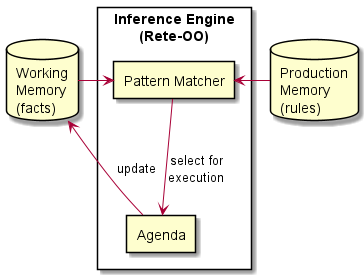
\includegraphics[width=0.55\textwidth]{Sections/images/components.png}}
    \caption{Drools components.}
    \label{fig:Drools_components}
\end{figure}

\begin{figure}[h]
    \centering
    \fbox{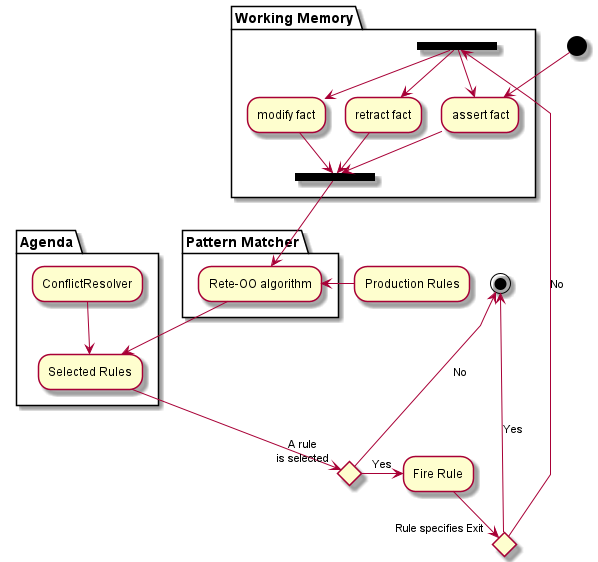
\includegraphics[width=0.55\textwidth]{Sections/images/InferenceLoop-1.png}}
    \caption{Drools Inference Loop.}
    \label{fig:Drools_inference_loop}
\end{figure}


The component we will be focussing on in this paper is the rules.
Rules are stored in a rules file, a text file, typically with a \.drl extension.  
During execution the rules do not change and are stored in production memory.
For the sake of this paper we will skip past package, import, global, declare, function and query, which are also stored in the rule file.
We will examine the anatomy of a rule.

A rule is made of 3 parts: attributes; conditions; and consequences.
Attributes are an optional hints to the inference engine as to how the rule should be examined.
The conditional, when, or left hand side (LHS) of the rule statement is a block of conditions that have to in aggregate return true for the asserted fact in order to be considered to be placed on the agenda.
The actions, consequences, then, or Right hand side (RHS) of the rule statement contains actions to be executed, should the rule be filtered

The LHS is a predicate statement, made up of a number of patterns.
variables can be bound to facts that match these patterns for use later in the LHS or for updating the working memory on the RHS.
the patterns are used to evaluate against the working memory.
The pattern match against the existence of facts.
Patterns can also match against conditions of the properties of facts.
Connectives such as not, and, and or can be applied to the patterns.
The patterns apply to individual Facts rather than the group, thus can be seen as first order predicates.

There are some more advanced features in the LHS, but for this paper, these are the features we will be looking at.

Whilst the RHS can contain arbitrary code to be executed when a rule is fired, it's main purpose is to adjust the state of truth in the working memory.
One can insert, modify, and retract facts in the working memory. 
modifying and retracting facts, must be done on fact variable references that have been created in the LHS.
One can explicitly terminate the inference loop, with a halt command.

\begin{figure}[h]
    \centering
    \fbox{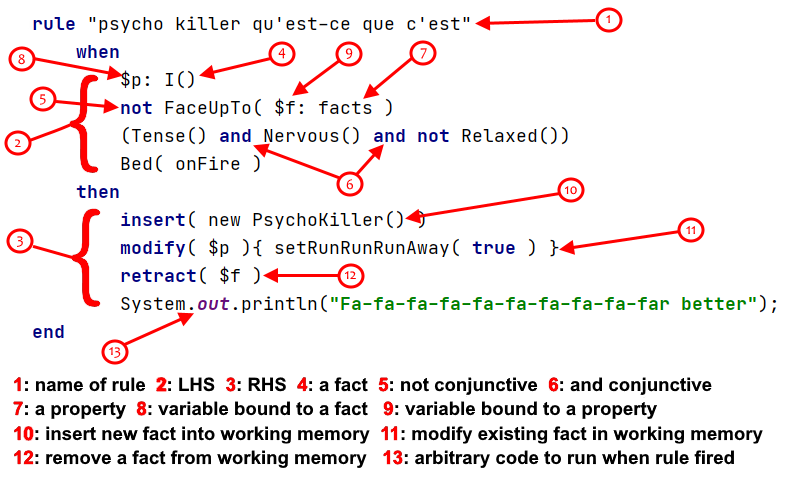
\includegraphics[width=0.95\textwidth]{Sections/images/DroolsRule2.png}}
    \caption{Drools Rule Breakdown.}
    \label{fig:Drools_Rule_Breakdown}
\end{figure}


\subsubsection{An explanatory example}
An example of a DRL file can be seen in listing \ref{listing:drl_file}.  This has been extracted from the Drools sample code. 

\begin{lstlisting}[language={[drl]Drools}, caption=Example Drools file., captionpos=b, label=listing:drl_file]
    package org.drools.examples.honestpolitician
 
    import org.drools.examples.honestpolitician.Politician;
    import org.drools.examples.honest politician.Hope;
     
    rule "We have an honest Politician"
        salience 10
        when
            exists( Politician( honest == true ) )
        then
            insertLogical( new Hope() );
    end
    
    rule "Hope Lives"
        salience 10
        when
            exists( Hope() )
        then
            System.out.println("Hurrah!!! Democracy Lives");
    end
    
    rule "Hope is Dead"
        when
            not( Hope() )
        then
            System.out.println( "We are all Doomed!!! Democracy is Dead" );
    end
    
    rule "Corrupt the Honest"
        when
            $p : Politician( honest == true )   
            exists( Hope() )
        then
            System.out.println( "I'm an evil corporation and I have corrupted " + $p.getName() );
            modify( $p ) { 
                setHonest( false ) 
            }
    end
\end{lstlisting}

Listing \ref{listing:drl_file} gives the Drools engine instructions on what actions to take when something changes in the working memory.
What this toy example does is reacts to when an honest politician is added to the working memory, prints a message celebrating the existence of said politician, corrupts her, gloats in a message and then prints a message of despair.
The code in listing \ref{listing:drl_file} does the following: 
\begin{enumerate}[topsep=2pt,itemsep=2pt,partopsep=2pt, parsep=2pt]
    \item on line 1 the package statement identifies the rule file
    \item on lines 3 and 4 the import statements describes which facts can be used
    \item the ``We have an honest Politician'' rule on line 6 does the following:
    \begin{enumerate}[topsep=2pt,itemsep=2pt,partopsep=2pt, parsep=2pt]
        \item using salience on line 7 it sets that this rule is to be run before rules with a lower salience
        \item on line 10 it checks the working memory for Politician facts with the honest property equal to true
        \item on line 12, if found then Hope facts will be inserted into the working memory
    \end{enumerate}
    \item the ``Hope Lives'' rule on line 15 does the following:
    \begin{enumerate}[topsep=2pt,itemsep=2pt,partopsep=2pt, parsep=2pt]
        \item line 18 check if any Hope facts exist
        \item on line 20, if found, it prints a message
    \end{enumerate}
    \item the ``Hope is Dead'' rule on line 23 does the following:
    \begin{enumerate}[topsep=2pt,itemsep=2pt,partopsep=2pt, parsep=2pt]
        \item checks if no Hope facts exist on line 25
        \item if none are found, on line 27, it prints a message 
    \end{enumerate}
    \item the ``Corrupt the Honest'' rule on line 30 does the following:
    \begin{enumerate}[topsep=2pt,itemsep=2pt,partopsep=2pt, parsep=2pt]
        \item line 32 checks for any Politician facts with the honest property equal to true, and sets them to the variable \$p
        \item line 33 checks if any Hope facts exist
        \item if both hope and politicians are found on line 35 it prints a message including the \$p variables name
        \item on line 36 to 38 it modifies the fact in working memory represented by \$p to change it's honest property 
    \end{enumerate}
\end{enumerate}